\section{\textbf{Methodology}}
\label{sec:methodology}
%%%%%%%%%%%%%% BASIC QUANTIZATION METHOD %%%%%%%%%%%%%%%%%%%%%%%%%%

\subsection{\textbf{Basic Quantization Method}}
\label{subsec:basic_notation}

Under \textit{uniform symmetric quantization} scheme, a real number $x$ is
uniformly mapped to an integer value $q \in [-2^{b-1}, 2^{b-1} - 1]$, where
$b$ specifies the quantization bit precision.
The formal definition is:
\begin{equation}
\label{eq:uniform_quantization}
\small
q = \mathrm{Q}(x, b, S) = \mathrm{Int}\bigg(\frac{\mathrm{clip}(x, -\alpha, \alpha)}{S}\bigg),
\end{equation}
where $\mathrm{Q}$ is the quantization operator, $\mathrm{Int}$ is the integer map (e.g., round to the nearest integer), $\mathrm{clip}$ is the truncation function, $\alpha$ is the
clipping parameter used to control the outliers, and $S$ is the scaling factor defined as $\alpha / (2^{b-1} - 1)$.
The reverse mapping from the quantized values $q$ to the real values (aka dequantization) is:
\begin{equation}
\small
\tilde{x} = \mathrm{DQ}(q, S) = Sq \approx x,
\end{equation}
where $\mathrm{DQ}$ denotes the dequantization operator. 
This approach is referred to as uniform symmetric quantization.
It is \textit{uniform} because the spacing between quantized values and their corresponding mapping to real
values is constant. However, several different non-uniform quantization methods have also been proposed~\cite{wu2016quantized, zhang2018lq, choi2018pact, park2018value}.
While non-uniform quantization approaches may better capture the distribution of parameters/activations than uniform quantization, they are in general difficult to deploy on hardware (as they often require a look up table which results in overhead).
Thus, we focus only on uniform quantization in this work.
In addition, this approach is \textit{symmetric} because we clip the values symmetrically within a range $[-\alpha, \alpha]$;
while in asymmetric quantization, the left and right side of this range could be asymmetric/different. 
Finally, we use \textit{static quantization} where all the scaling factors $S$ are fixed during inference to avoid runtime overhead of computing them. 
See~\sref{appendix:quantization_methods} for more details in quantization methods.



%%%%%%%%%%%%%% NON-LINEAR FUNCTIONS %%%%%%%%%%%%%%%%%%%%%%%%%%
\subsection{\textbf{ Non-linear Functions with Integer-only Arithmetic}}

The key to integer-only quantization is to perform all operations with integer arithmetic without using any floating point calculation.
Unlike linear (e.g., MatMul) or piece-wise linear operations (e.g., ReLU), this is not straightforward for non-linear operations (e.g., GELU, Softmax, and LayerNorm). 
This is because the integer-only quantization algorithms in previous works~\cite{yao2020hawqv3, jacob2018quantization} rely on the linear property of the operator.
For example, $\mathrm{MatMul}(Sq)$ is equivalent to $S\cdot \mathrm{MatMul}(q)$ 
for the linear MatMul operation.
This property allows us to apply integer MatMul to the quantized input $q$ and then multiply the scaling factor $S$ to obtain the same result as applying floating point MatMul to the dequantized input $Sq$. 
Importantly, this property \emph{does not} hold for non-linear operations, e.g., $\mathrm{GELU}(Sq) \not=S\cdot \mathrm{GELU}(q)$.
One na\"ive solution is to compute the results of these operations and store them in a look up table~\cite{lai2018cmsis}. 
However, such an approach can have overhead when deployed on chips with limited on-chip memory,
and will create a bottleneck proportional to how fast the look up table could be performed.
Another solution is to dequantize the activations and convert them to floating point, and then compute these non-linear operations with single precision logic~\cite{zafrir2019q8bert, bhandare2019efficient}.
However, this approach is not integer-only and cannot be used on specialized efficient hardware that does not support floating point arithmetic, e.g., ARM Cortex-M~\cite{armcortexm}.

To address this challenge, we approximate non-linear activation functions, GELU and Softmax, with polynomials that can be computed with integer-only arithmetic.
Computing polynomials consists of only addition and multiplication, 
which can be performed with integer arithmetic.
As such, if we can find good polynomial approximations to these operations, then we can perform the entire inference with integer-only
arithmetic. 
For instance, a second-order polynomial represented as $a(x+b)^2+c$ can be efficiently calculated with integer-only arithmetic as shown in~\aref{alg:intpoly}.\footnote{In~\aref{alg:intpoly}, $\floor{\cdot}$ means the floor function. Note that, $q_b$, $q_c$, and $S_{out}$ can be pre-computed under static quantization. That is to say, there is no floating point calculation, e.g., of $S/b$, in inference.}


%%%%%%%%%%%%%%%%%%%%%%%%%%%%%%%%%%%%%%%%%%%%%%%%%%%%%%%%%%%%%%%%%%%%%%%%

\begin{algorithm}[tb]
\caption{\footnotesize
   Integer-only Computation of Second-order Polynomial $a(x + b)^2 + c$}
\label{alg:intpoly}
\small
\begin{algorithmic}
\STATE {\bfseries Input:} $q, S$: quantized input and scaling factor 
\STATE {\bfseries Output:} $q_{out}, S_{out}$: quantized output and scaling factor
\vskip 0.075in
\FUNCTION{\textsc{I-Poly}$(q, S)$ 
\hspace*{\fill}{$\triangleright$ $ qS = x$}
}{  
    \STATE $q_b \leftarrow \floor{b / S}$ 
    \STATE $q_c \leftarrow \floor{c / aS^2}$
    \STATE $S_{out} \leftarrow \floor{aS^2}$
    \STATE $q_{out} \leftarrow (q + q_b)^2 + q_c$ 
    \STATE \Return $q_{out}, S_{out}$
    \hspace*{\fill}{$\triangleright$ 
    $ q_{out}S_{out} \approx  a(x + b)^2 + c\enspace$}

   }
\ENDFUNCTION
\end{algorithmic}
\end{algorithm}

%%%%%%%%%%%%%% POLYNOMIAL APPROXIMATION %%%%%%%%%%%%%%%%%%%%%%%%%%

\subsection{\textbf{Polynomial Approximation of Non-linear Functions}}

There is a large body of work on approximating a function with a polynomial~\cite{stewart1996afternotes}.
We use a class of \textit{interpolating polynomials}, where we are given
the function value for a set of  $n+1$ different data points $\{(x_0, f_0),\dots, (x_n, f_n)\}$, and we seek
to find a polynomial of degree at most $n$ that exactly matches the function value at these points.
It is known that there exists a unique polynomial of degree at most $n$ that passes through all the data points~\cite{waring1779vii}.
We denote this polynomial by $L$, defined as:
\begin{equation}
\label{eqn:lagrange}
\small
L(x) = \sum_{i=0}^{n} f_i l_i(x) \enspace \text{\upshape where} \enspace 
l_i(x) = \prod_{\substack{0 \le j \le n \\ j \ne i}} \frac{x - x_j}{x_i - x_j}.
\end{equation}

Interestingly for our problem, we have two knobs to change to find the best polynomial approximation.
Since we know the actual target function and can query its exact value
for any input,
we can choose the interpolating point $(x_i, f_i)$ to be any point on the function.
The second knob is to choose the degree of the polynomial.
While choosing a high-order polynomial results in smaller error (see Appendix~\ref{sec:error_of_lagrange}), there are two problems with this.
First, high-order polynomials have higher computational and memory overhead.
Second, it is challenging to evaluate
them with low-precision integer-only arithmetic,
as overflow can happen when multiplying integer values. For every multiplication, we need
to use double bit-precision to avoid overflow.
As such, the challenge is to find a good low-order polynomial that can closely approximate the
non-linear functions used in Transformers. 
This is what we discuss next, for GELU and Softmax, in~\sref{subsection:gelu} and~\ref{subsection:softmax}, respectively, where we show that one can
get a close approximation by using only a second-order~polynomial.




%%%%%%%%%%%%%%%%%%%%%%%%%%%% GELU %%%%%%%%%%%%%%%%%%%%%%%%%%%%%%%%%%
\subsection{\textbf{Integer-only GELU}}
\label{subsection:gelu}

GELU~\cite{hendrycks2016gaussian} is a non-linear activation function used in Transformer models, defined~as:
\begin{equation}
\small
\begin{split}
\label{eq:gelu}
    \mathrm{GELU}(x) &:= x \cdot \frac12 \left[ 1 + \mathrm{erf}(\frac{x}{\sqrt{2}})\right], \\
    \text{where} \enspace \mathrm{erf}(x) &:= \frac{2}{\sqrt{\pi}}\int_0^x \exp{(-t^2)} dt.
\end{split}
\end{equation}
Here, $\mathrm{erf}$ is the error function. Figure~\ref{fig:gelu-exp} shows the behaviour of the GELU function (shown in red).
GELU has a similar behaviour as ReLU (shown in green) in the limit of large positive/negative values,
but it behaves differently near zero.
Direct evaluation of the integration term in $\mathrm{erf}$ is not computationally efficient.
For this reason, several different approximations have been
proposed for evaluating GELU. For example, \cite{hendrycks2016gaussian} suggests using
Sigmoid to approximate $\mathrm{erf}$:
\begin{equation}
\label{eqn:gelu-approx}
\small
\mathrm{GELU}(x) \approx x \sigma(1.702 x),
\end{equation}
where $\sigma(\cdot)$ is the Sigmoid function.
This approximation, however, is not a viable solution for integer-only quantization, as the Sigmoid itself is another non-linear function which requires
floating point arithmetic.
One way to address this is to approximate Sigmoid with the so-called
hard Sigmoid (h-Sigmoid) proposed by~\cite{howard2019searching} (designed in the context of efficient computer vision models) to obtain an integer-only approximation for GELU:
\begin{equation}
\small
\label{eqn:hgelu}
\mathrm{h{\text-}GELU}(x) := x\frac{\mathrm{ReLU6}(1.702x+3)}{6} \approx \mathrm{GELU}(x).
\end{equation} 
We refer to this approximation as h-GELU.
Although h-GELU can be computed with integer arithmetic, we observed that replacing GELU with h-GELU in Transformers results in a significant accuracy drop.
This is due to the large gap between h-GELU and GELU as depicted in~\tref{tab:sigmoid-approximation}.%
\footnote{Later in our ablation study, we show this can lead to accuracy degradation of up to 2.2 percentages, as reported in~\tref{tab:gelu_comparison}.}
Figure~\ref{fig:gelu-exp} (left) also shows the noticeable gap between those two functions. 


A simple way to address the above problem is to use polynomials to approximate GELU, by solving
the following optimization problem:
\begin{equation}
\small
\begin{split}
\label{eq:gelu_opt_objective}
    &\min_{a,b,c} \frac12\left\| \mathrm{GELU}(x) 
    - x \cdot \frac{1}{2} \left[ 1 + \mathrm{L}(\frac{x}{\sqrt{2}})\right]\right\|_2^2 , \\
    &\mathrm{s.t.} \quad L(x) = a(x+b)^2 + c,
\end{split}
\end{equation}
where $\mathrm{L}(x)$ is a second-order polynomial used to approximate the $\mathrm{erf}$ function. 
Directly optimizing~\eref{eq:gelu_opt_objective} results in a poor approximation since the definition domain of $\mathrm{erf}$ contains the entire real numbers. 
To address this, we only optimize $L(x)$ in a limited range since $\mathrm{erf}$ approaches to 1 ($-$1) for large values of $x$.
We also take advantage of the fact that $\mathrm{erf}$ is an odd function (i.e., $\mathrm{erf}(-x)=-\mathrm{erf}(x)$), and thus only consider approximating it in the positive
domain.
After finding the best interpolating points, i.e., $(x_i,f_i)$ in~\eref{eqn:lagrange}, and applying these adjustments we arrive at the following polynomial:
\begin{equation}
\label{eq:bestL_erf}
\small
    \mathrm{L}(x) = \mathrm{sgn}(x)\left[a(\mathrm{clip}(|x|, \max=-b)+b)^2 + 1\right],
\end{equation}
where $a=-0.2888$ and $b = -1.769$, and $\mathrm{sgn}$ denotes the sign function.
\footnote{Note that $L(x)$ is approximating GELU in the range of $[0, -b]$.}
Using this polynomial we arrive at i-GELU, the integer-only approximation for GELU, defined~as:
\begin{equation}
\label{eqn:igelu}
\small
\mathrm{i{\text-}GELU}(x) := x \cdot \frac{1}{2} \left[ 1 + \mathrm{L}(\frac{x}{\sqrt{2}})\right].
\end{equation}


%%%%%%%%%%%%%%%%%%%%%%%%%%%%%%%%%%%%%%%%%%%%%%%%%%%%%%%%%%%%%%%
\begin{figure}[]
\centering{
\centerline{
  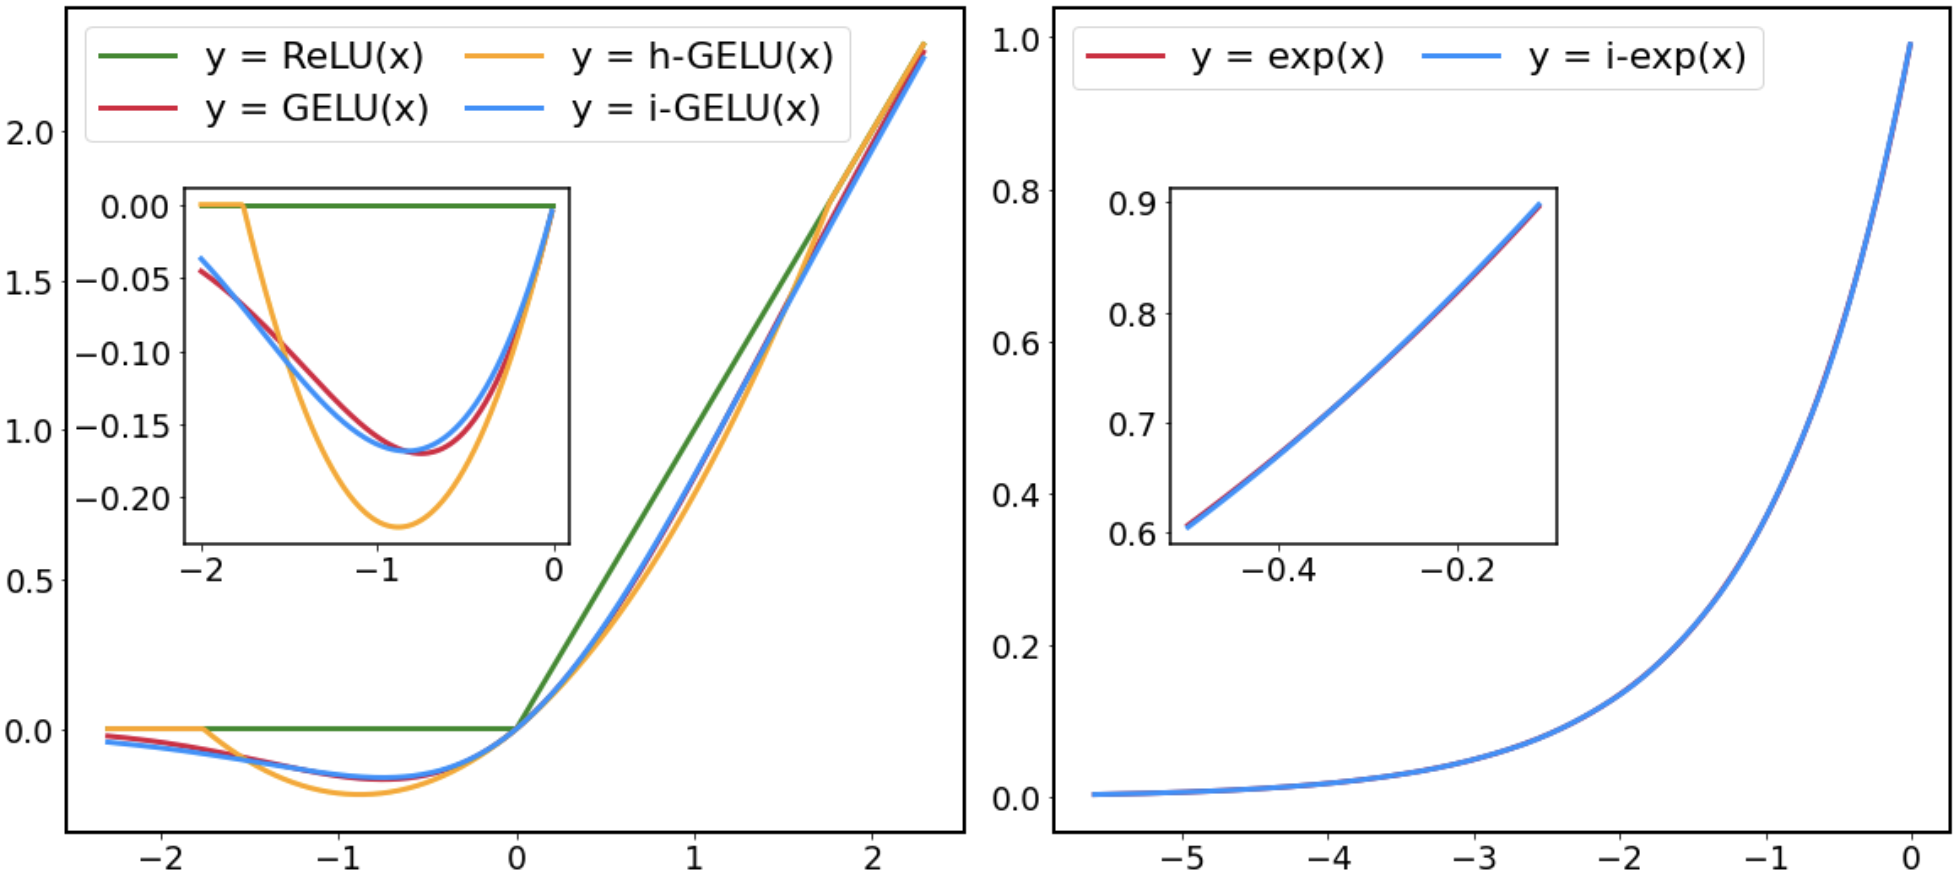
\includegraphics[width=0.48\textwidth]{figures/gelu-exp-approximation.png}
  }
  \caption{
  (Left) Comparison between RELU, GELU, h-GELU and i-GELU. 
  (Right) Comparison between exponential (exp) and our integer-only exponential (i-exp). 
  }
  \label{fig:gelu-exp}
  }
  \vspace{1mm}
\end{figure}
%%%%%%%%%%%%%%%%%%%%%%%%%%%%%%%%%%%%%%%%%%%%%%%%%%%%%%%%%%%%%%%

Algorithm~\ref{alg:intgelu} summarizes the integer-only computation of GELU using i-GELU.
We illustrate the behaviour of i-GELU in~\fref{fig:gelu-exp} (left). As one
can see, i-GELU closely approximates GELU, particularly around the origin.
We also report the approximation error of i-GELU along with h-GELU
in~\tref{tab:sigmoid-approximation}, where i-GELU has an
average error of $8.2 \times 10^{-3}$ and a maximum error of $1.8 \times 10^{-2}$.
This is $\sim3\times$ more accurate than h-GELU whose average and maximum errors are $3.1 \times 10^{-2}$ and $6.8 \times 10^{-2}$, respectively.
Also, i-GELU even slightly outperforms the Sigmoid based approximation of~\eref{eqn:gelu-approx}, but without using any floating point
arithmetic. 
Note that computing the Sigmoid requires floating~point.
Later in the results section, we show that this improved approximation, actually
results in better accuracy of i-GELU as compared to h-GELU (see~\tref{tab:gelu_comparison}).
 

%%%%%%%%%%%%%%%%%%%%%%%%%%%%%%%%%%%%%%%%%%%%%%%%%%%%%%%%%%%%%%%%%%%%%%%%

\begin{algorithm}[tb]
\caption{\footnotesize
Integer-only GELU }
\label{alg:intgelu}
\small
\begin{algorithmic}
\STATE {\bfseries Input:} $q, S$: quantized input and scaling factor  
\STATE {\bfseries Output:} $q_{out}, S_{out}$: quantized output and scaling factor 
\vskip 0.075in
\FUNCTION{\textsc{I-Erf}$(q, S)$
\hspace*{\fill}{$\triangleright$ $ qS = x$}
}{
    \STATE $a, b, c \leftarrow -0.2888, -1.769, 1$
    \STATE $q_{\mathrm{sgn}}, q 
    \leftarrow \mathrm{sgn}(q), \mathrm{clip}(|q|, \mathrm{max} = -b/S)$
    \STATE $q_{L}, S_{L} \leftarrow$ \textsc{I-Poly}${(q, S)}$ with $a, b, c$
    \hspace*{\fill}{$\triangleright$ \eref{eq:bestL_erf}$\enspace$}  
    \STATE $q_{out}, S_{out} \leftarrow q_{\mathrm{sgn}}q_L, S_L$ 
    \STATE \Return $q_{out}, S_{out}$
    \hspace*{\fill}{$\triangleright$ 
    $ q_{out}S_{out} \approx \mathrm{erf}(x)\enspace$}
   }
\ENDFUNCTION
 
\vskip 0.075in
\FUNCTION{\textsc{I-Gelu}$(q, S)$
\hspace*{\fill}{$\triangleright$ $ qS = x$}
}{
    \STATE $q_{\mathrm{erf}}, S_{\mathrm{erf}} \leftarrow$ \textsc{I-Erf}${(q, S / \sqrt{2})}$ 
    \STATE $q_{1} \leftarrow \floor{1/S_{\mathrm{erf}}}$
    \STATE $q_{out}, S_{out} 
    \leftarrow q(q_{\mathrm{erf}} + q_{1}), SS_{\mathrm{erf}}/2$
    \label{algline:geluapprox}
    \STATE \Return $q_{out}, S_{out}$
    \hspace*{\fill}{$\triangleright$ 
    $ q_{out}S_{out} \approx \mathrm{GELU}(x)\enspace$}
   }
\ENDFUNCTION
\end{algorithmic}
\end{algorithm}


%%%%%%%%%%%%%%%%%%%%%%%%%%%%%%%%%%%%%%%%%%%%%%%%%%%%%%%%%%%%%%%
\begin{table}[!t]
\vspace{-2mm}
\caption{ 
Comparison of different approximation methods for GELU. 
The second column (Int-only) indicates whether each approximation method can be computed with integer-only arithmetic.
As metrics for approximation error, we report L$^2$ and L$^\infty$ distance from GELU across the range of [-4, 4]. 
}

\vskip 0.1in
\label{tab:sigmoid-approximation}
\centering
\centerline{
\small{
\begin{tabular}{lccc}
\toprule
\ha                     & Int-only   & L$^2$ dist  & L$^\infty$ dist\\ 
\midrule              
\ha $x \sigma(1.702x)$  & \xmark              & 0.012                & 0.020                 \\
\ha h-GELU                & \cmark              & 0.031                & 0.068                 \\
\midrule                                              
\hc i-GELU (Ours)       & \cmark              & \bf{0.0082}          & \bf{0.018}            \\
\bottomrule
\end{tabular} 
}
}
\vspace{2mm}
\end{table}
%%%%%%%%%%%%%%%%%%%%%%%%%%%%%%%%%%%%%%%%%%%%%%%%%%%%%%%%%%%%%%%





%%%%%%%%%%%%%%%%%%%%%%%%%%%%%%%% SOFTMAX %%%%%%%%%%%%%%%%%%%%%%%%%%%%%%%%%%%%%%
\subsection{\textbf{Integer-only Softmax}}
\label{subsection:softmax}

Softmax normalizes an input vector and maps it to 
a probability distribution: 
\begin{equation}
\label{eqn:softmax} 
\small
\mathrm{Softmax}(\mathbf{x})_i := \frac{\exp{x_i}}{\sum_{j=1}^k \exp{x_j}} ,
\enspace \text{where} \enspace \mathbf{x} = [x_1, \dots, x_k].
\end{equation}
Approximating the
Softmax layer with integer arithmetic is quite challenging, as the exponential
function used in Softmax is unbounded and changes rapidly.
As such, prior Transformer quantization techniques~\cite{bhandare2019efficient,zafrir2019q8bert} treat this layer using floating point arithmetic.
Some prior work have proposed look up tables with interpolation~\cite{schraudolph1999fast},
but as before we avoid look up tables and strive for a pure arithmetic based approximation.
In addition, although \cite{hauser2001approximating} proposes polynomial approximation 
methods for the exponential function,
it uses significantly high-degree polynomials, and is only applicable on a limited finite domain. 

Similar to GELU, we cannot use a high-order polynomial, but even using such polynomial
is ineffective to approximate the exponential function in Softmax.
However, it is possible to address problem by limiting the approximation range of Softmax.
First, we subtract the maximum value from the input to the exponential for numerical stability:
\begin{equation}
\label{eqn:softmax2} 
\small
\mathrm{Softmax}(\mathbf{x})_i = \frac{\exp{(x_i - x_{\max})}}{\sum_{j=1}^k \exp{(x_j - x_{\max})}},
\end{equation}
where $x_{\max} = \max_i(x_i)$.
Note that now all the inputs to the exponential function, i.e., $\tilde x_i = x_i - x_{\max}$, become non-positive.
We can decompose any 
non-positive real number $\tilde x$ as $\tilde x = (-\ln{2})z + p$,
where the quotient $z$ is a non-negative integer and the remainder $p$ is a real number in $(-\ln2, 0]$. 
Then, the exponential of $\tilde x$ can be written as:
\begin{equation}
\label{eqn:expshift}
\small
\exp(\tilde x) = 2^{-z} \exp(p) = \exp(p) \verb|>>| z,
\end{equation}
where \verb|>>| is the bit shifting operation.
As a result, we only need to approximate the exponential function in the compact interval of $p\in(-\ln2, 0]$.
This is a much smaller range as compared to the domain of all real numbers.
Interestingly, a variant of this method was used in the Itanium 2 machine from HP~\cite{thomas2004libm,detrey2005parameterized}, but with a look up table
for evaluating $\exp(p)$.

We use a second-order polynomial to approximate the exponential
function in this range. To find the coefficients of the polynomial, we minimize the  L$^2$ distance from exponential function in the interval of $(-\ln2, 0]$. 
This results in the following approximation:
\begin{equation}
\label{eq:bestL_exp}
\small
L(p) = 0.3585 (p + 1.353)^2 + 0.344 \approx \exp(p). 
\end{equation}
Substituting the exponential term in~\eref{eqn:expshift} with this polynomial results in i-exp:
\begin{equation}
\label{eqn:iexp}
\mathrm{i\text{-}exp}(\tilde x) := L(p) \verb|>>| z  
\end{equation}
where $\enspace z = \floor{-\tilde x / \ln 2}$ and $p = \tilde x + z \ln 2$. This can be calculated with integer arithmetic.
Algorithm~\ref{alg:intexp} describes the integer-only computation of the Softmax fucntion using i-exp.
Figure~\ref{fig:gelu-exp} (right) plots the result of i-exp, 
which is nearly identical to the exponential function.
We find that the largest gap between these two functions is only $1.9 \times 10^{-3}$.
Considering that 8-bit quantization of a unit interval introduces a quantization error of $1/256 = 3.9 \times 10^{-3}$, our approximation error is relatively negligible and can be subsumed into the quantization error. 

%%%%%%%%%%%%%%%%%%%%%%%%%%%%%%%%%%%%%%%%%%%%%%%%%%%%%%%%%%%%%%%
\begin{algorithm}[tb]
\caption{\footnotesize
Integer-only Exponential and Softmax}
\label{alg:intexp}
\small
\begin{algorithmic}
\STATE {\bfseries Input:} $q, S$: quantized input and scaling factor  
\STATE {\bfseries Output:} $q_{out}, S_{out}$: quantized output and scaling factor
 
\vskip 0.075in
\FUNCTION{\textsc{I-Exp}$(q, S)$
\hspace*{\fill}{$\triangleright$ $ qS = x$}
}{
    \STATE $a, b, c \leftarrow 0.3585, 1.353, 0.344$
    \STATE $q_{\ln 2} \leftarrow \floor{\ln 2 / S}$
    \STATE $z \leftarrow \floor{-q / q_{\ln 2} }$
    \STATE $q_p \leftarrow q + z q_{\ln 2}$
    \hspace*{\fill}{$\triangleright$ $ q_pS = p\enspace$}
    \STATE $q_L, S_L \leftarrow$ \textsc{I-Poly}${(q_p, S)}$ with $a, b, c$
    \hspace*{\fill}{$\triangleright$ \eref{eq:bestL_exp}$\enspace$}
    \STATE $q_{out}, S_{out} \leftarrow q_L \verb|>>| z, S_L $
    \STATE \Return $q_{out}, S_{out}$    
    \hspace*{\fill}{$\triangleright$ 
    $ q_{out}S_{out} \approx \mathrm{exp}(x)\enspace$}
   }
\ENDFUNCTION
 
\vskip 0.075in
\FUNCTION{\textsc{I-Softmax}$(q, S)$
\hspace*{\fill}{$\triangleright$ $ qS = x$}
}{
    \STATE $\tilde q \leftarrow q - \mathrm{max}(q)$
    \STATE $q_{\mathrm{exp}}, S_{\mathrm{exp}} \leftarrow$ \textsc{I-Exp}${(\tilde q, S)}$  
    \STATE $q_{out}, S_{out} \leftarrow q_{\mathrm{exp}} / \mathrm{sum}(q_{\mathrm{exp}}), S_{\mathrm{exp}}$
    \STATE \Return $q_{out}, S_{out}$    
    \hspace*{\fill}{$\triangleright$ 
    $ q_{out}S_{out} \approx \mathrm{Softmax}(x)\enspace$}
   }
\ENDFUNCTION
\end{algorithmic}
\end{algorithm}


%%%%%%%%%%%%%%%%%%%%%%%%%%%%%%% LayerNorm %%%%%%%%%%%%%%%%%%%%%%%%%%%%%%%%%%%%%
\subsection{\textbf{Integer-only LayerNorm}}
\label{subsection:layernorm}

LayerNorm is commonly used in Transformers and involves several non-linear operations, such as division, square, and square root. 
This operation is used for normalizing the input activation across the channel dimension.
The normalization process is described as:
\begin{equation}
\label{eqn:lnmusigma}
\small
    \tilde{x} = \frac{x - \mu}{\sigma}  \enspace \text{\upshape where} \enspace
    \mu   =  \frac{1}{C}\sum_{i=1}^C x_i 
    \enspace \text{\upshape and} \enspace 
    \sigma = \sqrt{\frac{1}{C}\sum_{i=1}^C (x_i - \mu)^2}  .
\end{equation} 
Here, $\mu$ and $\sigma$ are the mean and standard deviation of the input across the channel dimension.
One subtle challenge here is that the input statistics (i.e., $\mu$ and $\sigma$) change
rapidly for NLP tasks, and these values need to be 
calculated dynamically during runtime. While computing
$\mu$ is straightforward, evaluating $\sigma$ requires the square-root
function.

The square-root function can be efficiently evaluated with integer-only
arithmetic through an iterative algorithm proposed in~\cite{crandall2006prime}, as described in~\aref{alg:intsqrt}.
Given any non-negative integer input $n$, this algorithm iteratively searches for the exact value of $\floor{\sqrt{n}}$ based on Newton's Method and only requires integer arithmetic.
This algorithm is computationally lightweight, as it converges within at most
four iterations for any INT32 inputs and each iteration consists only of one integer division, one integer addition, and one bit-shifting operation. 
The rest of the the non-linear operations in LayerNorm such as division and square are straightforwardly computed with integer arithmetic. 


%%%%%%%%%%%%%%%%%%%%%%%%%%%%%%%%%%%%%%%%%%%%%%%%%%%%%%%%%%%%%%%
\begin{algorithm}[tb]
\caption{\footnotesize
Integer-only Square Root }
\label{alg:intsqrt}
\small
\begin{algorithmic}
\STATE {\bfseries Input:} $n$: input integer 
\STATE {\bfseries Output:} integer square root of $n$, i.e., $\floor{\sqrt{n}}$
 
\vskip 0.075in
\FUNCTION{\textsc{I-Sqrt}$(n)$}{
    \STATE \textbf{if} $n=0$ \textbf{then return} $0$
    \STATE Intialize $x_0$ to $2^{\ceil{Bits(n)/2}}$ and $i$ to $0$
    \STATE \textbf{repeat}
    \STATE \hspace{10pt} $x_{i+1} \leftarrow \floor{(x_i + \floor{n / x_i}) / 2}$
    \STATE \hspace{10pt} \textbf{if} $x_{i+1} \ge x_i$  \textbf{then return} $x_i$
    \STATE \hspace{10pt} \textbf{else} $i \leftarrow i+1$
   }
\ENDFUNCTION
\end{algorithmic}
\end{algorithm} 